\documentclass[titlepage,openright,letterpaper,12pt]{book}
\usepackage{config/entete}
\usepackage{config/commandes} % Load les packages et définit des commandes.

%=============================================================================%

% On crée des bools qui sont False par défaut.
\newtoggle{VersionLivre}
\newtoggle{LivrePGChVide}
\newtoggle{ForceEntete}
\newtoggle{AuteureFemme}
\newtoggle{MemoirePasThese}
\newtoggle{useCustomFonts}
\newtoggle{generatePDFa}
\newtoggle{IntroConcluSansNombre}

% Switchboard, l'endroit ou on ajuste les toggles.
% Décommenté -> True; commenté -> False

%\toggletrue{VersionLivre}          % Décommenter pour faire la version livre
%\toggletrue{LivrePGChVide}         % Page gauche de chapiter vide en mode livre.
%\toggletrue{ForceEntete}            % Entête même pour version électronique.
%\toggletrue{AuteureFemme}          % Décommenter si l'auteur est une femme.
%\toggletrue{MemoirePasThese}       % Décommenter dans le cas d'un mémoire.
\toggletrue{IntroConcluSansNombre}  % Intro et conclusion non numérotées
\toggletrue{useCustomFonts}         % Fonts différents, voir switchboard.tex.
%\toggletrue{generatePDFa}           % Génère un PDFa plutôt qu'un PDF standard.

%=============================================================================%

\title          {Titre descriptif, pertinent et évocateur} % Pour la page de titre/jury.
\author         {Auteur(e)}  % Idem
\Organisation   {UNIVERSITÉ de SHERBROOKE}
\Location       {Sherbrooke, Québec, Canada}
\ResumeCourt    {On présente des résultats nouveaux dans un domaine en pleine effervescence.}
\date           {\today}       % Idem
\MotsClefs      {Mots-Clefs \sep Pertinents \sep avec séparateurs}

% On cache le code exécuté dans ce fichier parce qu'il est laid et impertinent.
\begin{comment}
\end{comment}

%=============================================================================%

\makeatletter   % Permet d'accèder aux variables @

%=============================================================================%

    % PDFA-1b/Hyperref
    \iftoggle{generatePDFa}
    {
        % PDF/A stuff (experimental)
        \usepackage[a-1b]{pdfx}
    }
    {
        \newcommand{\sep}{, }
    }%
        \begin{filecontents*}[overwrite]{\jobname.xmpdata}
\Title          {\@title}
\Author         {\@author}
\Subject        {\ResumeCourt}
\Org            {\Organisation}
\Keywords       {\MotsClefs}
\PublicationType{book}
        \end{filecontents*}%
        % Couleurs moins intenses, https://ethanschoonover.com/solarized/
        \definecolor{solblue}{HTML}{268bd2}
        \definecolor{solred}{HTML}{dc322f}
        \definecolor{solviolet}{HTML}{6c71c4}
        \definecolor{solmagenta}{HTML}{d33682}
        \definecolor{solcyan}{HTML}{2aa198}
        \definecolor{solorange}{HTML}{cb4b16}
        \definecolor{solyellow}{HTML}{b58900}
        \definecolor{solgreen}{HTML}{859900}
        % Hyperrefs
        \usepackage{hyperref}
        \hypersetup{
            pdfauthor={\@author},
            pdftitle={\@title},
            pdfsubject={\ResumeCourt},
            pdfkeywords={\MotsClefs},
            % pdfa,
            colorlinks=true,
            breaklinks=true,
            urlcolor=solmagenta,
            linkcolor=solblue,
            citecolor=solcyan,
            bookmarksopen=true,
            unicode=true
        }
        \usepackage[hyperpageref]{backref}      % Backrefs!
        \renewcommand{\backref}[1]{[cf.~p.~#1]} % Volé cette ligne à Samuel Boutin
        \usepackage{bookmark}
        \usepackage{cmap} % Doit être après hyperref pour être compatible avec pdf-a

%=============================================================================%

    \iftoggle{useCustomFonts}
    {   
        % Deux prochaines lignes -> Pagella et Mathpazo
        %\usepackage{mathpazo} % utilise Palatino pour les mathématiques (mettre en premier)
        %\usepackage{tgpagella} % utilise la police TeX Gyre Pagella

        % Deux prochaines lignes -> New Century et Fourier
        %\usepackage{newcent}
        %\usepackage{fouriernc}
        
        \usepackage{newcent}
        \usepackage{fouriernc}
        \renewcommand{\dagger}{\text{\textdagger}} % Millennial missing dagger fix
        \renewcommand{\iint}{\int\!\!\int}  % Better spacing
        \renewcommand{\iiint}{\int\!\!\int\!\!\int}
        \renewcommand{\iiiint}{\int\!\!\int\!\!\int\!\!\int}
    }
    {}

%=============================================================================%
    
    \iftoggle{AuteureFemme}
    { \newcommand{\monsieurMadame}{Mme.} }    
    { \newcommand{\monsieurMadame}{M.} }

%=============================================================================%

    \iftoggle{MemoirePasThese}
    {   % Si c'est un mémoire
        \newcommand{\documentPresente}{Mémoire présenté}
        \newcommand{\leDocument}{le mémoire}
        \newcommand{\leGrade}{maître ès science (M.Sc.)}
    }
    {   % Si c'est une thèse
        \newcommand{\documentPresente}{Thèse présentée}
        \newcommand{\leDocument}{la thèse}
        \newcommand{\leGrade}{docteur ès science (Ph.D.)}
    }

%=============================================================================%
    
    % Gestion de la version électronmique vs celle imprimée.
    \iftoggle{VersionLivre}
    {   % On fait la version imprimée!

        % On utilise un fontsize plus petit(10pt vs 12pt).
        \let\small\relax
        \let\footnotesize\relax
        \let\scriptsize\relax
        \let\tiny\relax
        \let\large\relax
        \let\Large\relax
        \let\LARGE\relax
        \let\huge\relax
        \let\Huge\relax
        \input{size10.clo}  % Ajuste le fontsize ET les marges
        \geometry{twoside=true, bottom=2.54cm} % L'ordre est important, pour les marges/fontsize.
        %\widowpenalty5000  % Décommenter s'il y a trop de ligne veuves/orphelines.
        %\clubpenalty5000   


        % On enlève la numérotation des pages vides
        \let\origdoublepage\cleardoublepage
        \newcommand{\clearemptydoublepage}{%
            \clearpage%
            {\pagestyle{empty}\origdoublepage}%
            }
        \let\cleardoublepage\clearemptydoublepage
        
        % Permet de mettre un page blanche seulement dans la version imprimée
        \newcommand{\autoPageBlancheLivre}{\clearpage\null\thispagestyle{empty}}

        \iftoggle{LivrePGChVide}
        {
            \let\stdchapter\chapter
            \renewcommand\chapter{\clearpage\null\thispagestyle{empty}\stdchapter}
            \renewcommand{\autoPageBlancheLivre}{}

            \let\stdpart\part
            \renewcommand\part{\clearpage\null\thispagestyle{empty}\stdpart}

            \renewcommand\@endpart{\vfil
                          \if@twoside
                            \null
                            \thispagestyle{empty}%
                            \newpage
                          \fi
                          \if@tempswa
                            \twocolumn
                          \fi}
        }{}

        % Les hyperliens n'ont pas desoins d'être colorés
        \hypersetup{hidelinks}
        % On affiche les DOI dans la biblio -> Pratique en version imprimée
        \bibliographystyle{config/nature-fr-showdoi}
        % On garde les entêtes dans la bibliographie
        \newcommand{\bibpagestyle}{}
    }
    {   % S'il y a un côté, on fait la version électronique.
        \geometry{letterpaper, lmargin=1.25in, rmargin=1.25in,
                  tmargin=1.5in, bmargin=1.0in, twoside=false}
        \iftoggle{ForceEntete}
        {
            % On garde les entêtes dans la bibliographie
            \newcommand{\bibpagestyle}{}
        }
        {
        % Prochaines lignes enlèvent l'entête
            \renewcommand{\chaptermark}[1]
                {\markboth{{\thechapter. #1}}{}}
            \renewcommand{\sectionmark}[1]{}
            % On enlève les entêtes dans la bibliographie
            \newcommand{\bibpagestyle}{\pagestyle{plain}}
        }

        % On n'affiche pas les DOI dans la biblio -> Plus propre
        \bibliographystyle{config/nature-fr}
        %\bibliographystyle{unsrt-fr} % unsrt partiellement traduit. Préférer nature.
        
        % Permet de mettre un page blanche seulement dans la version imprimée
        \newcommand{\autoPageBlancheLivre}{}
    }
    \iftoggle{IntroConcluSansNombre}
    {
        \newcommand{\Introduction}{\chapter*{Introduction}
            \addcontentsline{toc}{chapter}{Introduction}}
        \newcommand{\Conclusion}{\chapter*{Conclusion}
            \addcontentsline{toc}{chapter}{Conclusion}}
    }
    {
        \newcommand{\Introduction}{\chapter{Introduction}}
        \newcommand{\Conclusion}{\chapter{Conclusion}}
    }


%=============================================================================%

\makeatother    % Plus d'accès aux variables @


%=============================================================================%

\begin{document}

%=============================================================================%
% Titre
\begin{comment}
\end{comment}
\makeatletter   % Permet d'accèder aux variables @

\thispagestyle{empty}  % Page blanche avec formattage manuel
\pagenumbering{gobble} % Aucune numérotation, sinon hypperref bug
\vglue 2cm
\begin{center}
    \doublespacing{
    {\LARGE \@title}\\
    \vspace{2.0cm}
    par\\
    \vspace{2.0cm}
    {\large \@author}
    \vspace{2.0cm}\\
    \documentPresente\ au département de physique\\
    en vue de l'obtention du grade de \leGrade
    \vfill
    FACULTÉ des SCIENCES\\
    \Organisation\vspace{1.0cm}\\
    \Location, \@date  % La date sera celle de la compilation
    }
\end{center}

\makeatother    % Plus d'accès aux variables @


\frontmatter % Pagination de préambule

% Jury
\begin{comment}
\end{comment}
\makeatletter   % Permet d'accèder aux variables @

\iftoggle{LivrePGChVide}
{}
{
    % Next two lines force a linebreak in ebook versions
    \chapter*{}
    \vspace{-4.7cm}
}

\thispagestyle{empty}

\begin{center}
    \vglue 2cm
    % Le \underline{\hspace{5cm}}\\ 
    %Le \@date % Lorsque le document sera accepté!
    \vspace{2cm}
    \scalebox{1} % Empêche le retour à la ligne si le nom est trop long.
    % {\it le jury a accepté \leDocument\ de \monsieurMadame~\@author~dans sa version finale.} 
    
    \vspace{1cm}
    Membres du jury\\
    \vspace{1cm}

    Professeur Stefanos Kourtis\\
    Directeur de recherche\\
    Département de physique\\
    \vspace{1cm}

    Professeur Guillaume Duclos-Cianci\\
    Co-directeur de recherche\\
    Département de physique\\
    \vspace{1cm}
    
    Professeur Alexandre Blais\\
    Membre interne\\
    Département de physique\\
    \vspace{1cm}

    Professeur David Sénéchal\\
    Président rapporteur\\
    Département de physique\\
    \vspace{1cm}

    Professeur Gilles Zémor\\
    Membre externe\\
    Université de Bordeaux\\
    \vspace{1cm}
\end{center}

%\clearpage

\makeatother    % Plus d'accès aux variables @


% Dédicace
\begin{comment}
\end{comment}

\chapter*{}
\vspace{-10pt}
\begin{flushright}
    À \underline{\hspace{4cm}}
\end{flushright}

\thispagestyle{empty}

% Sommaire
\clearpage  % Mets le sommaire à la bonne page dans la TOC
\chapter*{Sommaire}
\addcontentsline{toc}{chapter}{Sommaire}
\begin{comment}
\end{comment}

C'est ouvrage traite principalement de la protection de
l'information. 
Pas au sens que nous entendons souvent dans les médias de protection des renseignements privés,
mais plutôt au sens de robustesse face à la corruption des données.
En effet,
lorsque nous utilisons un cellulaire pour envoyé un texto,
plusieurs facteurs, 
comme les particules atmosphériques et l'interférence avec d'autres signaux,
peuvent modifier le message initial.
Si nous ne faisons rien pour protéger le signal,
il est peu problable que le contenu du texto reste inchangé
lors de la réception.

C'est ce problème qui a motivé le premier projet 
de recherche de cette thèse.
Sous la supervision du professeur David Poulin,
j'ai étudié une généralisation des codes polaires,
une technologie au coeur du protocol de communication de 5ième génération (5G).
Pour cela,
j'ai utilisé les réseaux de tenseurs, 
des outils mathématiques initialement développé pour étudier
les matériaux quantiques.
L'avantage de cette approche est qu'elle permet une représentation
graphique intuitive du problème, 
ce qui facilite grandement le développement des algorithmes.

Cette idée d'utiliser des outils mathématiques graphiques pour 
étudier des problèmes de protection de l'information
sera le fil conducteur pour le reste de la thèse.
Cependant, 
pour la suite, 
les erreurs n'affecteront plus des systèmes de communications classiques,
mais plutôt des systèmes de calcul quantique.
Et, comme nous le verrons dans cette thèse,
les systèmes quantiques sont naturellement beaucoup plus sensible aux erreurs.

À cet effet, 
j'ai effectué un stage au sein de l'équipe de Microsoft Research,
principalement sous la supervision de Micheal Beverland, 
lors duquel j'ai conçu des circuits permettant de mesurer un système quantique afin d'identifier
les potentiels fautes qui affectent celui-ci.
J'ai également proposée une architecture qui permetterait d'implémenter ces circuits
de façon réaliste en laboratoire.
Finalement, avec le reste de l'équipe, 
nous avons prouver mathématiquement que les circuits que j'ai développés sont optimaux.
L'ensemble de ces résultats sont inspirés de méthodes issues de la théorie des graphes.

J'ai terminé ma thèse sous la supervision du professeur Stefanos Kourtis.
Avec celui-ci,
j'ai créé une méthode, toujours basée sur une approche graphique, 
qui permet d'automatiquement concevoir de nouveaux protocoles de 
corrections des erreurs dans un système quantique.
Cela nous a permis de montrer qu'il est probablement beaucoup plus facile 
que ce que le croyait la communauté scientifique de concevoir de tels protocoles.

Vous aurez remarqué que lors de tous ces projets,
je n'ai jamais eu le même superviseur.
C'est pour cela que je qualifie ma thèse d'odyssée.
Celle-ci a été parsemée d'embuches.
D'abord avec le triste départ trop rapide du professeur David Poulin.
C'est suite à cela que j'ai postulé pour un stage au sein de l'équipe de Microsoft
dans le but d'avoir une nouvelle supervision.
Cependant, le stage c'est finalement déroulé en virtuel après avoir été repousssé
plusieurs fois en raison de la pandémie.
C'est après ce stage que je me suis finalement greffé à l'équipe du professeur Kourtis 
qui venait de démarrer son groupe.
Heureusement,
lors de toutes cette étape, 
je pouvais toujours compter sur le soutien de Guillaume Duclos-Ciani,
initialement professionel de recherche au sein du groupe de David Poulin.

En bref,
j'espère que vous aurez du plaisir à lire cette thèse même si celle-ci 
tire un peu dans tous les sens.
Elle réflète les connaissances et compétences que j'ai acquéries en travaillant sous 
la supervision de plusieurs mentors en plus de s'intéresser à l'un des problèmes
parmi les plus importants pour la réalisation des promesses de l'informatique quantique.

Bonne lecture!


% Remerciements
\chapter*{Remerciements}
\begin{comment}
\end{comment}

\kant[2-3] % Remplissage



% Tables des matières/Figures
{
    \setlength{\parskip}{0ex}
    \tableofcontents
    \listoffigures
    %\listoftables
}

%=============================================================================%

\mainmatter % Pagination standard
\onehalfspacing

%-----------------------------------------------------------------------------%

% \include serait préférable à \input à partir d'ici, mais MiKTeX sur Windows
% n'aime pas les \cite dans un \include. Fonctionne parfaitement sur TeXLive.

\begin{comment}
\end{comment}

\Introduction   % Chapitre qui ne sera pas numéroté si IntroConcluSansNombre est Vrai

L'ordinateur et l'internet figurent parmi les technologies qui ont le plus impacté
notre mode de vie et l'organisation de nos sociétés.
En effet,
il est désormais possible d'accéder à une quantité phénoménale de connaissance,
de connecter avec une personne de l'autre côté du globe
et d'automatiser les taches du quotidient.
Tout cela avec une efficience qui peut sembler sans limite.

Cependant, 
bien que ces technologies offrent des performances impressionantes,
il existe des taches pour lesquelles le temps nécessaire peut s'approche ou
dépasse l'age actuel de l'univers.
Bien sur,
le temps d'exécution dépend de la taille de la tache a effectuer.
Par contre, 
la difficulté de différentes taches n'augmente pas de manière similaire.

Par exemple,
il sera deux fois plus long pour un ordinateur d'inverser l'ordre d'une liste 
si la longueur de cette dernière est doublée.
Par contre,
il ne suffit que d'ajouter un chiffre à un nombre pour que celui-ci soit deux 
fois plus long à factoriser~\cite{arora_computational_2009}.
Formellement,
on dit que la complexité du premier problème augmente linéairement avec la taille de l'entrée,
alors que celle du second problème augmente exponentiellement.

Les problèmes dont la complexité augmente exponentiellement requierent donc un temps de calcul
hors de porté, et ce, même pour des instances de tailles modestes.
Par contre,
cette façon de calculer la complexité suppose un modèle de calcul dit classique,
soit le modèle utilisé par les ordinateurs actuels.
Et,
comme vous vous en doutez probablement si vous lisez cette thèse,
le modèle de calcul classique n'est pas le seul modèle de calcul.

L'idée du calcul quantique est attribuée à Ed Fredkin et Richard Feynman et 
c'est ce dernier qui aurait présenté cette possibilité en 1981 lors d'une conférence au MIT~\cite{hoofnagle_birth_2021}.
Depuis,
le calcul quantique a fait beaucoup de chemin,
nottament après une publication de Peter Shor dans laquelle il introduit un 
algorithme pouvant factoriser un nombre avec une complexité polynomiale selon
le nombre de chiffres à l'aide d'un ordinateur quantique~\cite{shor_algorithms_1994}.
Dans ce cas,
doubler la longueur du nombre de fait que multiplier par huit le temps de calcul.
Cela est beaucoup plus efficace que la croissance exponentielle requise par un ordinateur classique.

Bien que ce résultat ne permet pas de résoudre tous les problèmes dont la complexité classique
est exponentielle,
il démontre tout de même que certains problèmes,
qui semblaient hors d'atteintes des ordinateurs classiques,
sont en théorie résolubles, en un temps raisonnable, par un ordinateur quantique.
Cela a bien sûr suscité un fort engouement pour l'information quantique et
il existe aujourd'hui des applications dans plusieurs domaines comme
la cryptographie~\cite{bennett_quantum_2014, gisin_quantum_2002}, 
la chimie~\cite{lanyon_towards_2010, mcardle_quantum_2020, cao_quantum_2019} 
et l'optimisation~\cite{montanaro_quantum_2016, grover_quantum_1997}.
En plus de cela,
il existe fort probablement plusieurs autres applications qui nous sont encore inconnues.

Ainsi,
l'informatique quantique a le potentiel de repousser les frontières de ce qui est ajourd'hui
possible pour le recherche scientifique.
Cependant,
pour réaliser de tels promesses,
il faut d'abord construire un ordinateur quantique capable d'exécuter ces nouveaux algorithmes quantiques.
Et cela,
bien évidemment,
n'est pas une tache simple.

Plusieurs technologies sont proposées pour construire les ordinateurs quantiques.
Que ce soit les circuits supraconducteurs~\cite{wallraf_strong_2004, krantz_quantum_2019}
la photonique quantique~\cite{obrien_photonic_2009, kok_linear_2007},
les points quantiques~\cite{pioro-ladriere_electrically_2008, loss_quantum_1998}
ou l'une des nombreuses autres approches proposées,
toutes ces technologies apportent leur lot de défis.
Plusieurs de ces enjeux,
comme le choix des matériaux ou
des méthodes de couplage et de contrôle
sont unique a une ou quelques approches.
Cependant,
un obstacle majeur à lequel toutes ces technologies sont confrontés
est la décohérence des systèmes quantiques~\cite{unruh_maintaining_1995, palma_quantum_1996}.

La décohérence apparait lorsqu'un système quantique peut intéragir avec son environnement
et elle se manifeste sous plusieurs formes, 
comme la perte de photons ou la relaxation du système vers un état d'énergie inférieure.
Cela engendre donc des erreurs lors du calcul quantique,
ce qui éloigne les résultats obtenus de ceux désirés.
Puisqu'il essentiel d'intéragir avec un système quantique pour exécuter les diverses 
opérations nécessaires à l'informatique quantique,
la présence des erreurs est inévitable.

Heureusement,
il est possible de corriger les erreurs plus vites qu'elles apparaissent~\cite{aharonov_fault-tolerant_1999}.
La correction des erreurs lors du calcul quantique est le sujet de cette thèse.
Dans celle-ci,
je présenterai les résultats de trois projets adressant cet enjeu.
L'ordre de présentation des résultats suit l'augmentation du réalisme du modèle étudié à chaque section.

Dans le premier chapitre,
je présenterai un projet sur la correction d'erreurs dans les systèmes classiques.
L'étude des systèmes classiques permet de développer une intuition qui est également
applicable aux systèmes quantiques.
De plus, il s'agit de problèmes ayant plusieurs applications en télécommunication.
Nottament,
les systèmes que j'ai étudiés,
soient les codes polaires convolutifs,
sont une généralisation des codes polaires,
une méthode au coeur des technologies de communication de cinquième génération (5G)~\cite{arikan_rate_2009, bioglio_design_2021}.
Les travaux que j'ai effectué ont permis d'identifier les paramètres qui maximisent la réduction des erreurs
en fonction du temps de calcul nécessaire pour la correction.

Dans le deuxième chapitre,
je ferai en premier pas vers le régime quantique.
Dans celui-ci,
j'utiliserai un modèle simplifier de génération des erreurs sur un système quantique.
Cela permet de se concentrer sur la construction de codes correcteurs,
un outil essentiel à la réalisation du calcul quantique protégé des erreurs.h
Ainsi,
je montrerai dans ce chapitre une nouvelle approche de construction de codes correcteurs
basée sur des méthodes de résolution de problèmes de satisfaction de contraintes,
des méthodes d'informatique théorique classique grandement étudiées~\cite{arora_computational_2009, noauthor_minizinc_nodate, noauthor_sat_nodate, achlioptas_rigorous_2005}.
Cette approche permet alors d'identifier des régimes pour lesquels il est beaucoup plus simple qu'espéré
de construire des codes correcteurs.
De plus,
les résultats numériques présentés montrent que les codes construits de cette manière
sont optimaux pour le modèle de bruit étudié.

Dans le troisième chapitre,
j'introduirai un modèle de calcul quantique,
soit la réalisation d'une mémoire quantique.
En effet,
sans avoir a effectué des opérations précises,
il est déjà difficile de protéger un système quantique lorsque celui-ci est inactif.
Ce modèle,
d'apparence simple,
permet tout de même de développer et d'étudier plusieurs outils qui seront nécessaires
au calcul quantique plus général.
Dans ce chapitre,
j'utiliserai des méthodes de la théorie des graphes pour designer une architecture 
permettant d'implémenter une mémoire quantique en laboratoire.
De plus,
je montrerai que les approches proposées minimisent le nombre d'opérations nécessaires
et qu'elles permettent de construire des ordinateurs quantiques de grandes échelles.

Les modèles étudiés dans cette thèse sont tous agnostiques du choix de technologie de qubit.
Ce choix se justifie de deux façons.
Premièrement,
chacune des technologies présentement considérées ont des avantages et des inconvénients variés.
Il est encore tôt pour sélectionner la meilleure technologie qui sera utilisée pour réaliser
tous les ordinateurs quantiques.
Ainsi, il est pertinent de développer des modèles et méthodes universelles.
Deuxièmement,
bien qu'il reste beaucoup de défis à relevés pour implémenter physiquement des méthodes
de correction d'erreurs sur des ordinateurs quantiques,
des résultats récents montrent qu'il est possible d'adapter les méthodes agnostiques
aux choix technologiques.
De plus,
prendre en considération des réalités expérimentales,
telles que des biais dans le bruit~\cite{tuckett_ultrahigh_2018}
ou des détails sur l'implémentation des qubits~\cite{noh_fault-tolerant_2020, darmawan_practical_2021},
semble généralement améliorer les performances des méthodes de correction des erreurs.

Les chapitres de la thèse se présentent tous de la même façon.
Il débute par une introduction haut niveau au modèle de bruit qui sera étudié.
Cette introduction est suivit d'une exposition des outils mathématiques nécessaires à
la compréhension des résultats.
Les résultats sont présentés à la fin de chaque chapitre sous la forme d'un article.
Au premier et troisième chapitre,
l'article présenté a été revu par des pairs et est publié dans un journal.
L'article du deuxième chapitre était encore en révision au moment de soumettre la thèse.

\begin{comment}
\end{comment}

\chapter{Théorie}

%-----------------------------------------------------------------------------%

% Ce qui suit n'est que du remplissage avec un petit exemple de ref/eqref
\section{Section}
\subsection{Exemple math \label{sec:newton}}

Newton a reçu -- ou pas -- une pomme sur la tête avant de déterminer, dans \cite{newton1687philosophiae}, que
\begin{align}
    \label{eq:newton}
    \vec F=m \vec a,
\end{align}
son équation la plus célèbre. Comme on le voit donc à l'équation~\eqref{eq:newton} de la section~\ref{sec:newton}, la force est proportionnelle à l'accélération.

On peut aussi exprimer la mécanique sous la forme lagrangienne. Pour des coordonnées généralisées $q$ et leur dérivées $\dot q$, le lagrangien est alors

\begin{align}
    \label{eq:lagrangien}
    L(q, \dot q, t) = T - V
\end{align}

et les équations du mouvement dérivent des équations de Lagrange 

\begin{align}
    \label{eq:equations_lagrange}
    \frac{\partial L}{\partial q} - \frac{\mathrm{d}}{\mathrm{d}t}\frac{\partial L}{\partial \dot q} = 0 \quad \forall q
    .   % Fin de la phase -> point
\end{align}

Ainsi, bien que ça ne soit pas évident de prime abord, les équations~\eqref{eq:newton} et~\eqref{eq:equations_lagrange} sont conceptuellement équivalentes!

\subsection{Exemple citation}
Citons aussi un vieil article \cite{andreev1964} et un autre \cite{robertson1929}. Maintenant citons les deux à la fois \cite{andreev1964, robertson1929}. Ensuite, citons plusieurs références avec un commentaire chacunes \cites[p.~1]{robertson1929}[chap.~2]{andreev1964}[\textsection 6]{newton1687philosophiae}. Finalement, citons les mêmes références, mais ne mettons des commentaires que lorsque nécessaire \cites{robertson1929}[chap.~2]{andreev1964}{newton1687philosophiae}.

\subsection{Parenthèses ajustables}
Voici des exemples d'utilisantion des paranthèses ajustables définies dans le package \emph{commandes}\footnote{Voici comment faire une note en bas de page. Voir le fichier \texttt{commandes.sty} pour des commandes personnalisées et personnalisables.}:
\begin{align}
    a&=\p{123}            \\
    a&=\p[]{123}          \\
    a&=\p[big]{123}       \\
    a&=\pc[Big]{123}      \\
    a&=\pc[bigg]{123}     \\
    a&=\pa[Bigg]{123}     \\
    a&=\pa[none]{123}     \\
    a&=\moy{\int t\dd t}  \\
    a&=\norm{\int t\dd t} \\
    a&=\abs[Bigg]{123}    \\
\end{align}

\subsection{Remplissage}
\kant[8-10]


\begin{comment}
\end{comment}

\chapter{Résultats}

%-----------------------------------------------------------------------------%

\section{Exemple de graphique}

La figure~\ref{fig:phdcomics} est très drôle, sérieusement.

\begin{figure}[htb]
    \begin{center}
        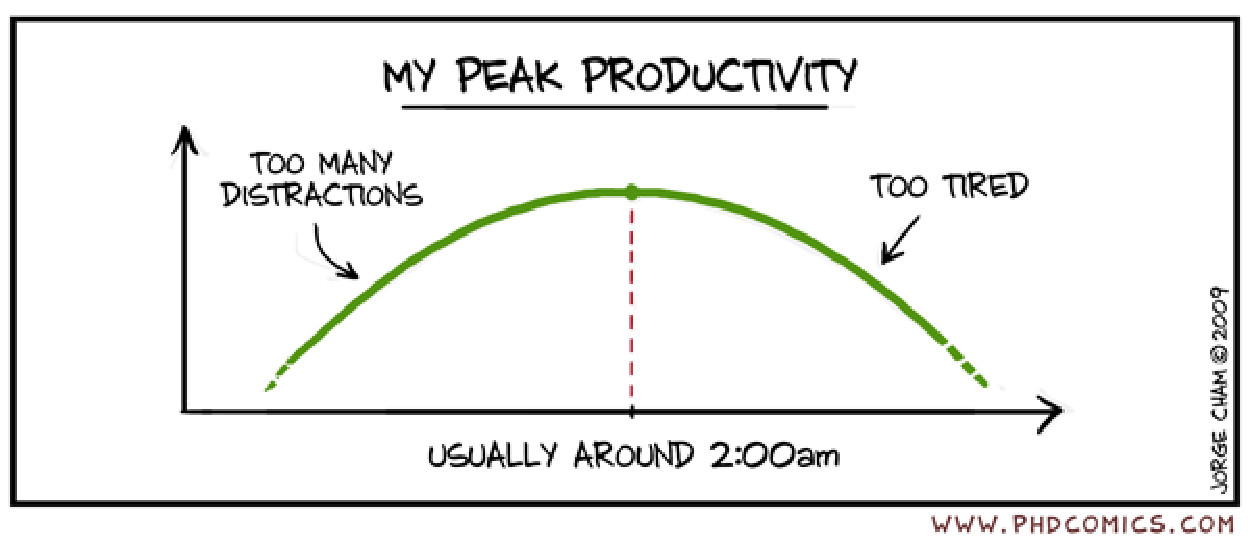
\includegraphics[width=0.8\columnwidth]{figures/phd083109s.pdf} 
        \longcaption{Figure à la fois hilarante et véridique.}{Image tirée du webcomic "Piled Higher and Deeper" par Jorge Cham \href{www.phdcomics.com}{www.phdcomics.com}. Seule la première partie de ce long caption sera dans la table des figures.}
        \label{fig:phdcomics}
    \end{center}
\end{figure}

\section{Remplissage}
\kant[11-14]

\begin{comment}
\end{comment}

\Conclusion % Chapitre qui ne sera pas numéroté si IntroConcluSansNombre est Vrai

Dans cette thèse,
j'ai présenté trois projets de recherche effectués lors de mon doctorat.
Tous ces projets traitent de la correction des erreurs,
mais dans des modèles de calcul différents.

Lors du premier projet,
j'ai mesuré l'impact de divers paramètres sur la performance et le temps de décodage
des codes polaires convolutifs.
Cela a permis d'identifier que les codes de profondeur et largeur deux offrent les
meilleures performances en fonction du temps de décodage.
Ce résultat pousse donc plus loin les performances des codes polaires standards
qui sont présentement utilisés dans le réseau de communication 5G.
Bien que les considérations d'ingénierie d'un réseau de communication sortent du cadre de cette thèse,
il est évident que toutes les améliorations à la correction d'erreurs peuvent réduire les 
couts d'implémentation d'un tel réseau.
En effet,
comme le taux d'erreur dépend de la distance entre les antennes,
un code qui permet de corriger plus d'erreurs permet également d'augmenter la distance
entre les antennes ce qui engendre une réduction du nombre nécessaire.

Le second projet que j'ai présenté est en réalité le dernier que j'ai effectué.
Dans le cadre de celui-ci,
je me suis intéressé à la construction de codes correcteurs quantiques.
La contribution la plus importante de ce projet réside dans la connexion
entre les problèmes de satisfaction de contraintes et la construction de codes.
Cela a permis de numériquement démontrer l'existence d'un seuil de satisfaisabilité
pour la probabilité d'inclusion d'une arête dans le graphe de support,
au-delà duquel il est facile de trouver des codes.
Il existe donc des régimes de paramètres pour lesquels il est aisé de construire des codes.
De plus,
j'ai poussé la méthode plus loin pour construire une famille de codes LDPC offrant des 
performances optimales pour le canal à effacement.
Il reste encore du chemin à faire,
mais cette approche offre la possibilité de découvrir des codes correcteurs pouvant être
adaptés aux contraintes physiques des ordinateurs quantiques à court et moyen terme.

Le troisième projet dont j'ai traité s'intéresse à la réalisation d'une architecture
permettant l'implémentation d'une mémoire quantique.
Des simulations numériques montrent également que cette approche permet de réduire significativement
le nombre de qubits nécessaires.
Bien sûr,
il reste de nombreux défis à résoudre pour implémenter cette architecture en laboratoire,
notamment l'implémentation de connexions à longue portée entre les qubits.
Tout de même,
l'approche présentée permet d'éliminer les croisements entre les connexions en exploitant
un petit nombre de couches dans la troisième dimension.
De plus,
les méthodes de traçage de graphes utilisées pour obtenir cette architecture 
ont le potentiel d'être appliquées pour contourner d'autres limitations à l'implémentation
du calcul tolérant aux fautes.

Dans l'ensemble de ces projets,
les modèles de bruits étudiés demeurent agnostiques de la technologie utilisée pour construire
les qubits.
Ce choix est fait puisqu'il est encore trop tôt pour choisir une technologie parmi toutes celles
proposées.
Il reste donc du travail à faire pour adapter les méthodes proposées dans cette thèse aux diverses 
technologies de qubits.
Cependant,
les travaux de cette thèse démontrent bien comment il est possible d'utiliser divers outils,
des réseaux de tenseurs aux méthodes de traçage de graphes en passant par les problèmes de satisfaction
de contraintes,
pour faciliter le design de systèmes quantiques tolérant aux fautes.

%-----------------------------------------------------------------------------%

\singlespacing

\begin{comment}
\end{comment}

\appendix
% \renewcommand\chapterstring{Annexe}

\chapter{Théorie de l'information}
\label{chap:theo_info}

Considérant une variable aléatoire $X$ dont les valeurs possibles sont les éléments de $\mathcal X$
avec probabilité $\Pr: \mathcal X \to [0, 1]$,
la quantité d'information acquise après une réalisation $x \in \mathcal X$ de cette variable
est $\log(1/\Pr(x))$.
L'\textbf{entropie de Shannon} est l'espérance de cette valeur, soit 
\begin{align}
  H(X) = \mathbb E\qty(\log\qty(\frac{1}{\Pr(X)})) = -\sum_{x\in\mathcal X}\Pr(x) \log(\Pr (x)).
\end{align}
Dans cette définition,
il est considéré que $p\log(p) = 0$ lorsque $p = 0$.

Pour deux variables aléatoires $X, Y$ de domaines $\mathcal X, \mathcal Y$,
l'\textbf{entropie conjointe} est 
\begin{align}
  H(X, Y) 
  = \mathbb E\qty(\log\qty(\frac{1}{\Pr(X, Y)})) 
  = -\sum_{x\in\mathcal X, y \in\mathcal Y}\Pr(x, y) \log(\Pr(x, y))
\end{align}
et l'\textbf{entropie conditionnelle} est
\begin{align}
  H(X | Y) 
  = \mathbb E\qty(\log\qty(\frac{1}{\Pr(X|Y)})) 
  = -\sum_{x\in\mathcal X, y \in\mathcal Y}\Pr(x, y) \log(\Pr(x|y)).
\end{align}
Il est aisé de vérifier que 
\begin{align}
  H(X, Y) = H(X | Y) + H(Y) = H(Y | X) + H(X).
\end{align}
Ainsi,
l'information acquise après la réalisation simultanée de deux variables aléatoires
est équivalente à la somme de l'information acquise en réalisant la première 
et de l'information acquise en réalisant la seconde en connaissant la valeur de la première.

L'\textbf{information mutuelle} entre deux variables aléatoires $X, Y$ est
l'information que révèle une réalisation d'une des variables sur l'autre variable.
L'information mutuelle se mesure en comparant la probabilité conjointe de $X, Y$
aux probabilités marginales, soit
\begin{align}
  I(X ; Y) 
  &= \mathbb E\qty(
    \log\qty(\frac{1}{\Pr(X)\Pr(Y)})
    -
    \log\qty(\frac{1}{\Pr(X, Y)})
  ) \notag \\
  &= -\sum_{x\in\mathcal X, y \in\mathcal Y}\Pr(x, y) \log(\frac{\Pr(X, Y)}{\Pr(X)\Pr(Y)}).
\end{align}
Cette définition est symétrique,
c'est-à-dire $I(X ; Y) = I(Y ; X)$.
De plus,
l'information mutuelle est reliée aux diverses entropies selon
\begin{align}
  I(X;Y)
  = H(X) - H(X | Y)
  = H(Y) - H(Y | X)
  = H(X) + H(Y) - H(X, Y).
\end{align}
Le première équation illustre bien que l'information mutuelle correspond à la différence
d'information acquise par une réalisation de $X$ lorsque $Y$ est inconnue ou connue.


\chapter{Théorie des graphes}
\label{chap:theo_graphe}

Un \textbf{graphe} est une paire $(S, A)$ telle que 
\begin{align}
  A \subseteq \qty{\qty{s, t} : s,t \in S}.
\end{align}
Les éléments de $S$ se nomment \textbf{sommets}
et les éléments de $A$ se nomment \textbf{arêtes}.
Deux sommets $s, t \in S$ sont \textbf{connectés} si $\qty{s, t} \in A$.
Le \textbf{voisinage} d'un sommet $s$ est l'ensemble des arêtes contenant $s$,
soit 
\begin{align}
  \eta(s) = \qty{a \in A : s \in a}.
\end{align}
Le \textbf{degré} d'un sommet est la taille de son voisinage.

Un \textbf{graphe biparti} est un graphe pour lequel il existe une 
partition des sommets $S = U \cup V$ telle que 
\begin{align}
  A \subseteq \qty{\qty{u, v} : u \in U,\, v \in V}.
\end{align}
Ainsi, les arêtes sont restreintes entre les paires de sommets n'appartenant pas
au même ensemble.
Un \textbf{hypergraphe} est une généralisation d'un graphe
où le nombre de sommets par arête est arbitraire.
Ainsi,
un hypergraphe est une paire $(S, A)$ telle que
\begin{align}
  A \subseteq \qty{X \subseteq S}.
\end{align}
Le voisinage et le degré d'un sommet sont définis de façon similaire à un graphe.
De plus, le poids $|a|$ de $a \in A$ est le nombre de sommets de cette arête.

Il existe une correspondance entre les graphes bipartis et les hypergraphes.
Pour un hypergraphe $H = (S, A)$,
la fonction 
\begin{align}
  \phi(H) = (S \cup A, B),
\end{align}
avec $\qty{s, a} \in B$ si $s \in a$,
est bijective et associe à chaque hypergraphe un unique graphe biparti.

Un \textbf{cycle} de longueur $n$ est un graphe $C_n = (S, A)$
avec $S = \qty{s_1, s_2, \ldots, s_n}$ et 
$A = \qty{\qty{s_1, s_2}, \qty{s_2, s_3}, \ldots, \qty{s_n, s_1}}$.
Un cycle de longueur paire est un graphe biparti.

Soit deux graphes $G = (S, A)$ et $H = (T, B)$,
le \textbf{produit cartésien} $G \times H$ est un graphe $(S \times T, C)$
tel que $\qty{(s_1, t_1), (s_2, t_2)} \in C$ si 
$s_1 = s_2$ et $\qty{t_1, t_2} \in B$ ou si $t_1 = t_2$ et $\qty{s_1, s_2} \in A$.
Le produit cartésien de deux graphes contenant chacun deux sommets et une arête reliant ces
sommets est un cycle de longueur quatre.
Ainsi,
pour le produit cartésien $G \times H$,
chaque paire d'arêtes $a \in A$ et $b \in B$ engendre un cycle de longueur quatre dans $C$.

\chapter{Complexité de calcul}
\label{chap:complexite_calcul}

Dans cette section,
la rigueur des définitions est variable.
Définir formellement la complexité de calcul demande d'introduire un modèle de 
calcul comme la machine de Turing.
Cependant,
cela sort beaucoup du cadre de cette thèse
et je me contente de définitions qui sont suffisantes à la compréhension du contenu de la thèse
et j'évite plusieurs détails.

Un \textbf{problème de calcul} est représenté par une relation $R \subseteq X \times Y$, 
où $X$ est l'ensemble des \textbf{entrées} et $Y$ est l'ensemble des \textbf{solutions}.
Les solutions de $x \in X$ sont les éléments de l'ensemble $Y_R(x) = \qty{y \in Y : (x, y)\in R}$.
Un \textbf{algorithme} $a: X \to Y$ résout $R$ si $a(x) \in Y_R(x)$ pour tous $x \in X$.

Un algorithme se décompose en une série d'opérations $a_1, \ldots a_c \in \mathcal A$ telle
que $a(x) = (a_c \circ \ldots \circ a_1)(x)$ où $\circ$ représente la composition
de fonctions.
Cette décomposition de $a$ varie en fonction de la taille de $x$
et dépend également des opérations accessibles $\mathcal A$.
Plus précisément,
il est supposé que les entrées $X$ sont décrites par des listes de tailles variées
d'éléments d'un alphabet $\mathcal X$.
Ainsi,
$X \subseteq \mathcal X^* = \cup_{n=0}^\infty \mathcal X^n$ et
une entrée $x \in X$ a une taille $n$ si $x \in \mathcal X^n$.

La \textbf{complexité} d'un algorithme est le nombre $c(n)$ d'opérations nécessaires
pour calculer $a(x)$ selon la taille $n$ de $x$.
Il est souvent difficile et peu pertinent de calculer la valeur exacte de $c(n)$
et il est généralement suffisant de connaitre le comportement général de $c(n)$.
Pour ce faire,
nous utilisons la \textbf{notation grand $\mathcal O$}.
Une fonction $f(n)$ a la complexité $\mathcal O(g(n))$ s'il existe
une constante $k$ telle que $f(n) \leq k g(n)$.
Généralement,
les complexités considérées sont les complexités \textbf{logarithmiques} $\mathcal O(\log n)$,
\textbf{linéaire} $\mathcal O(n)$,
\textbf{polynomiale} $\mathcal O(n^t)$ pour un entier $t > 0$
et \textbf{exponentielle} $\mathcal O(2^n)$.

Par exemple,
le problème du tri d'une liste d'entiers est défini par la relation
$R \subseteq \mathbb Z^* \times \mathbb Z^*$
où chaque paire $(x, y) \in R$ est une liste $x$ et sa version triée $y$.
Les opérations disponibles pour trier une liste sont la permutation et
la comparaison de deux éléments.
Comme il y a $n(n-1)/2$ paires de nombre,
un algorithme naif de tri a une complexité $\mathcal O(n^2)$.

Dans cette thèse,
j'utilise trois classes de complexité importantes.
Premièrement,
la \textbf{classe P} est l'ensemble des problèmes
pour lesquels il existe un algorithme de complexité polynomiale.
Deuxièmement,
la \textbf{classe NP} est l'ensemble des problèmes
pour lesquels il existe un algorithme de complexité polynomiale
qui permet de vérifier qu'une paire $(x, y)$ satisfait la relation.
La différence avec la classe P est qu'il n'est pas nécessaire qu'un 
algorithme de complexité polynomial soit en mesure de trouver $y \in Y_R(x)$,
mais seulement qu'un algorithme soit en mesure de vérifier que $y$ est une solution
de $x$.
Troisièmement,
un problème de la \textbf{classe $\sharp$P} est défini à partir d'un problème
$R = (X, Y)$ de la classe NP.
Le problème $N = (X, Y_R(X))$ de $\sharp$P correspondant est le problème de
recherche du nombre de solutions dans $R$ d'une entrée $x \in X$.

Évidemment, $\text{P} \subseteq \text{NP}$.
Par contre, 
il est toujours une question ouverte de déterminer si
$\text{P} \subset \text{NP}$ ou si $\text{P} = \text{NP}$.
Par contre,
la conjecture la plus acceptée est que $\text{P} \subset \text{NP}$.

Un problème $R = (X_R, Y)$ est \textbf{complet} pour une classe de complexité
si pour tout problème $S = (X_S, Y)$ de cette classe il existe une fonction 
$f: X_S \to X_R$ de complexité polynomiale.
En particulier,
un problème $R$ est \textbf{NP-complet} si un algorithme $A$ pour $R$
permet de construire, avec un surcout polynomial,
un algorithme pour résoudre un problème arbitraire de NP.

\chapter{Théorie des groupes}
\label{chap:theo_groupes}

Un \textbf{groupe} $(G, *)$ est un ensemble $G$ avec une opération $* : G \times G \to G$
satisfaisant les trois conditions suivantes.
L'opération $*$ est associative.
Il existe un élément identité $e$ tel que $e * g = g * e = g$ pour tous $g \in G$.
Chaque élement $g \in G$ a un inverse $g^{-1} \in G$ tel que $g * g^{-1} = g^{-1} * g = e$.
Par exemple $(\mathbb Z, +)$ est le groupe des nombres entiers avec l'opérateur d'addition.
De plus, un groupe est \textbf{abélien} si l'opération est commutative.

Les groupes considérés dans la thèse sont tous des groupes multiplicatifs.
Dans ce cas, l'opérateur est noté $\cdot$ et régulièrement omis.
Ainsi, $gh$ et $g \cdot h$ sont deux notations équivalentes pour la multiplication 
de deux éléments d'un groupe.
Comme l'opération est sous-entendu,
il est commun de noter un groupe $(G, \cdot)$ seulement à partir de l'ensemble $G$.

La \textbf{cardinalité} $|G|$ d'un groupe $G$ est le nombre d'éléments de celui-ci.
Les groupes considérés dans la thèse ont tous une cardinalité finie.
Un \textbf{sous-groupe} est un sous-ensemble $H \subseteq G$ satisfaisant les trois conditions
d'un groupe.
Je note alors $H \sqsubseteq G$.
Un sous-ensemble $S \subseteq G$ est un \textbf{générateur} d'un sous-groupe $H$ si $H$ est le plus petit
sous-groupe contenant $S$.
J'utilise $g(H)$ pour représenter un générateur de $H$ 
et $\langle S \rangle$ pour représenter le sous-groupe généré par $S$.
Les éléments d'un sous-ensemble $S \subseteq G$ sont \textbf{indépendants} si 
$|\langle T \rangle| < |\langle S \rangle|$ pour tous $T \subset S$.

Pour $H \sqsubseteq G$,
la \textbf{classe à gauche} d'un élément $g \in G$ est
\begin{align}
  gH = \qty{gh : h \in H}.
\end{align}
De même,
la \textbf{classe à droite} de $g$ est 
\begin{align}
  Hg = \qty{hg : h \in H}.
\end{align}
Si $Hg = gH$ pour tous $g \in G$,
alors $H$ est un \textbf{sous-groupe normal} et,
pour tous $f, g \in G$, l'opération
\begin{align}
  (fH)\cdot(gH) = (fg)H
\end{align}
entre les classes de $H$ respecte la définition d'un groupe.
Cela permet de former le \textbf{groupe quotient} 
\begin{align}
  G / H = \qty{gH : g \in G},
\end{align}
soit le groupe des classes de $H$.

La \textbf{conjugaison} de $g \in G$ et $H \sqsubseteq G$ est 
\begin{align}
  gHg^{-1} = \qty{ghg^{-1} : h \in H}.
\end{align}
Le \textbf{normalisateur} de $H$ est l'ensemble des éléments de $G$ qui laisse $H$
invariant après conjugaison.
C'est-à-dire, l'ensemble
\begin{align}
  \mathcal{N}_G(H) = \qty{g \in G : gHg^{-1} = H}.
\end{align}
Le \textbf{centralisateur} de $H$ est l'ensemble des éléments de $G$ qui commutent avec
tous les éléments de $H$, soit
\begin{align}
  \mathcal{C}_G(H) = \qty{g \in G : gh = hg,\, h \in H}.
\end{align}
Il est toujours vrai que $\mathcal{C}_G(H) \subseteq \mathcal{N}_G(H)$ puisque
si $g \in \mathcal{C}_G(H)$ alors $ghg^{-1} = hgg^{-1} = h$.

Soit un groupe $G$ tel que $fg = \pm gf$ pour tous $f,g \in G$
et $H \sqsubseteq G$ tel que $h \in H \implies -h \not\in H$,
alors $\mathcal{N}_G(H) = \mathcal{C}_G(H)$ puisque
\begin{align}
  ghg^{-1} = \pm hgg^{-1} = \pm h = h
\end{align}
pour tous $h \in H$.
Ceci est le cas pour le groupe stabilisateur présenté au chapitre~\ref{chap:construction_codes}
de cette thèse.


%=============================================================================%

% Voir switchboard.tex pour le bibliographystyle selon le type de document.
\bibliography{references}        % Le fichier de bibliographie est memoire.bib.

\end{document}
